\section*{Les maquettes}
\addcontentsline{ptc}{section}{Les maquettes}
\label{sec:maquettes}

Voici les différentes maquettes du site :

\begin{figure}[!h]
    \centering
    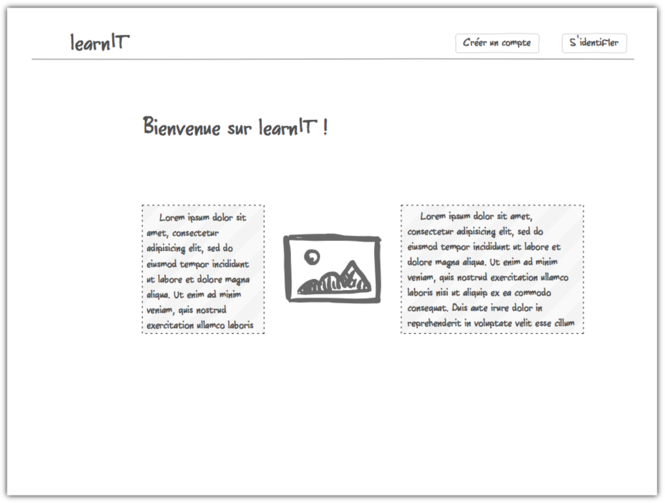
\includegraphics[scale=1]{textures/images/annexes/maquettes/1a-Home.png}
    \caption{La page d'accueil}
\end{figure}
\begin{figure}[!h]
    \centering
    \includegraphics[scale=1]{textures/images/annexes/maquettes/1b-CréerCompte.png}
    \caption{La page d'inscription}
\end{figure}

\newpage

\begin{figure}[!h]
    \centering
    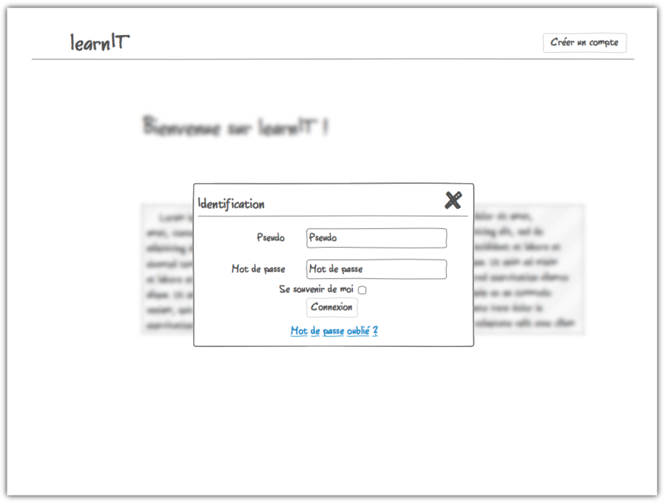
\includegraphics[scale=1]{textures/images/annexes/maquettes/1c-Sidentifier.png}
    \caption{La page de connexion}
\end{figure}
\begin{figure}[!h]
    \centering
    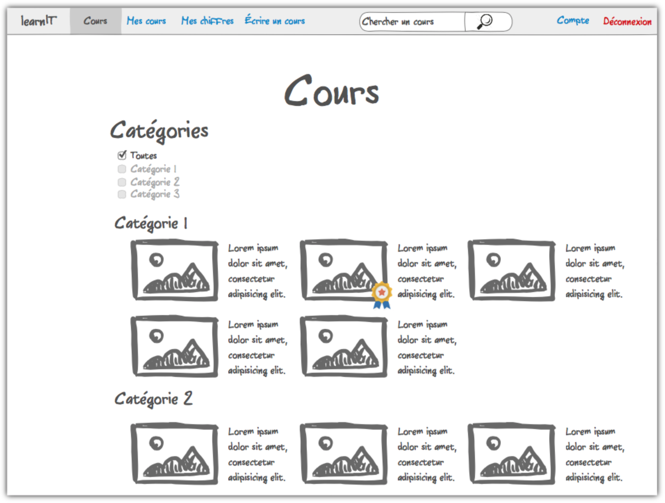
\includegraphics[scale=1]{textures/images/annexes/maquettes/2-Cours.png}
    \caption{La liste des cours}
\end{figure}

\newpage

\begin{figure}[!h]
    \centering
    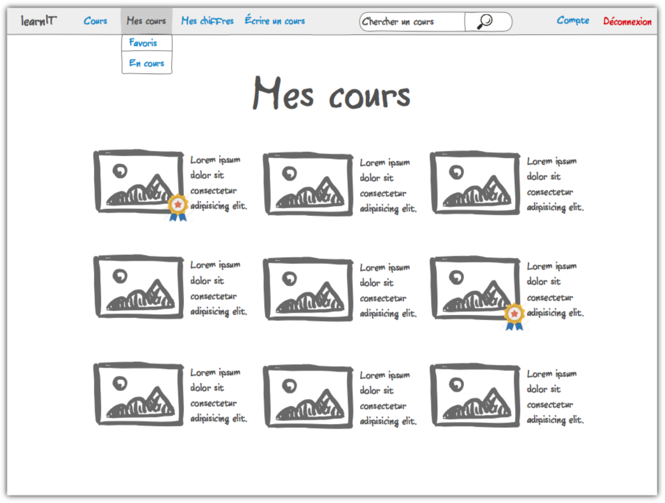
\includegraphics[scale=1]{textures/images/annexes/maquettes/3-MesCours.png}
    \caption{La liste des cours auxquels l'utilisateur est inscrit}
\end{figure}
\begin{figure}[!h]
    \centering
    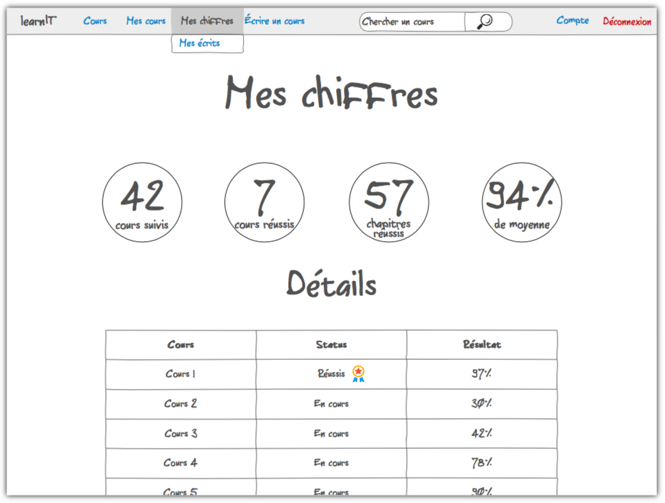
\includegraphics[scale=1]{textures/images/annexes/maquettes/4-MesChiffres(Cours).png}
    \caption{La page des chiffres}
\end{figure}

\newpage

\begin{figure}[!h]
    \centering
    \includegraphics[scale=1]{textures/images/annexes/maquettes/5-ÉcrireCours.png}
    \caption{La page de création d'un cours}
\end{figure}
\begin{figure}[!h]
    \centering
    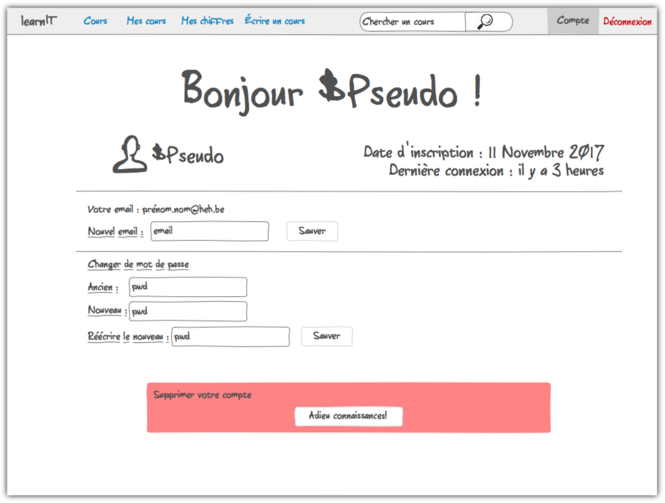
\includegraphics[scale=1]{textures/images/annexes/maquettes/6-Compte(utilisateur).png}
    \caption{La page du compte utilisateur}
\end{figure}